\chapter{Cameras, Shader Graphs, and Rendering Budgets}

\section{A Camera Is a Map}

Chapter 7 ended with a limit: a statement such as \emph{the arrangement has six quadruple points} is a statement about a model, and no single image certifies it. This chapter asks what a camera does to a model, how a shader graph can attach data to what the camera sees, and what an image costs. As in Chapter 7 the measurements were made with Blender's Python module, version $5.2.2$, run headless with the Eevee engine under software rendering, and the scripts named in the text are part of the evidence.

A perspective camera is a map from points of space to points of a rectangle. With the camera at the origin looking down its own negative $Z$ axis, a point with camera coordinates $(x,y,z)$, $z<0$, lands on the sensor at
\[
  u = f\,\frac{x}{-z},\qquad v = f\,\frac{y}{-z},
\]
where $f$ is the focal length in millimetres, and the sensor coordinates are converted to pixels by the number of pixels per millimetre. Blender's default sensor fit applies the sensor width, $36$ mm, to the longer side of the frame, so for a frame $W\times H$ with $W\ge H$ the scale is $W/36$ pixels per millimetre, and for a portrait frame the same sensor width is applied to $H$. The horizontal field of view of a landscape frame is $2\arctan\bigl(36/(2f)\bigr)$, which is $73.74^\circ$ at $24$ mm, $39.60^\circ$ at $50$ mm, and $23.91^\circ$ at $85$ mm. An orthographic camera drops the division by depth: points are projected along the view axis and scaled by a single orthographic scale, which is the width of the visible region in scene units. The depth division is the whole difference. Under it, two equal spheres at different distances appear at different sizes, and under the orthographic map they appear at the same size.

\lstinputlisting[language=Python,basicstyle=\ttfamily\footnotesize,breaklines=true,frame=single,columns=fullflexible,keepspaces=true,firstline=14,lastline=22]{camera_probe.py}

The formula is testable against rendered pixels. The script \texttt{camera\_probe.py} places five small emissive spheres at known points, renders a $400\times300$ frame with the world black, locates each sphere's centroid by connected-component analysis, and compares that with three predictions: the function above, Blender's own \texttt{world\_to\_camera\_view}, and the centroid after adding half a pixel for the pixel-centre convention. At $24$, $50$, and $85$ mm the largest distance between a predicted position and a measured centroid was $0.12$, $0.06$, and $0.06$ pixels, and the function above agreed with \texttt{world\_to\_camera\_view} to better than $10^{-4}$ pixel. The orthographic camera agreed with its prediction to $0.08$ pixel, and a $300\times400$ portrait frame, in which the sensor width governs the vertical side, agreed to $0.06$ pixel. The tests show that the textbook formula is the camera Blender implements, including the half-pixel convention and the sensor-fit rule, and a reader who needs to place an annotation, a label, or a measurement in an image can compute its position rather than reading it off by eye.

\section{What One View Can Certify}

An orthographic view of a sphere shows the points of its near hemisphere. For a vertex on the unit sphere with outward direction $\mathbf v$ and a view direction $\mathbf d$ pointing from the sphere toward the camera, the vertex is on the near side exactly when $\mathbf v\cdot\mathbf d>0$, and the number $\mathbf v\cdot\mathbf d$, the cosine of the angle between the two, is the \emph{facing}. A vertex near the limb has small facing and is foreshortened, so its marker is an ellipse seen edge-on and is easily hidden by a tube, as the readback of Chapter 7 found.

The vertex sets of the two arrangements of Chapter 11 are centrally symmetric. Every circle is a great circle, so if $\mathbf v$ lies on a set of circles then $-\mathbf v$ lies on the same set. It follows that for any direction $\mathbf d$ that is not perpendicular to a vertex, exactly half the vertices face the camera, and the measurement agrees: with $4000$ view directions spread evenly over the sphere, the script's arrangement showed $13$ of its $26$ vertices in every view and the teaching arrangement showed $27$ of $54$. The orthographic image is therefore blind to exactly half of the vertices at every moment, and a count of coloured markers in one image bounds the count for the model by a factor of two at best.

Two views from opposite sides see every vertex once. The practical question is how much margin they leave. Taking the facing of $0.2$ used in Chapter 7 as the threshold below which a marker is unreliable, the number of vertices above threshold in a single view varied from $8$ to $13$ (median $10$) for the script's arrangement and from $18$ to $26$ (median $22$) for the teaching arrangement. For an antipodal pair, the search over $4000$ directions found nine directions at which every vertex of the script's arrangement has $|\mathbf v\cdot\mathbf d|>0.2$, and none for the teaching arrangement, whose best pair leaves a smallest facing of $0.157$. A third view cures this: a greedy selection showed that three views suffice for both arrangements at the threshold $0.2$. The result is a design rule with a number attached, and it depends on the arrangement, because the teaching arrangement has more vertices to place away from a limb.

The geometric prediction was then compared with the ray-cast of Chapter 7, which includes the globe and the tubes. At the best antipodal direction, the surface bound found every vertex of the script's arrangement reachable in the two views, $13+13=26$, and every vertex of the teaching arrangement, $27+27=54$. The stricter centre bound, which asks for an unobstructed ray to the marker centre, certified $10+10=20$ and $19+19=38$. The gap between the bounds is the same phenomenon as in Chapter 7: markers seen obliquely can be partly covered by neighbouring tubes. Figure 8.1 shows the antipodal pair for the script's arrangement. In both images the markers are emissive and keep their assigned colours, but the surface and tubes in the left image are lit weakly because the two lights are fixed in the world, not attached to the camera. The lesson for a figure that will be compared across views is to fix the lights relative to the camera, or to accept that shading will differ between views and not to rely on it as data.

\begin{figure}[ht]
\centering
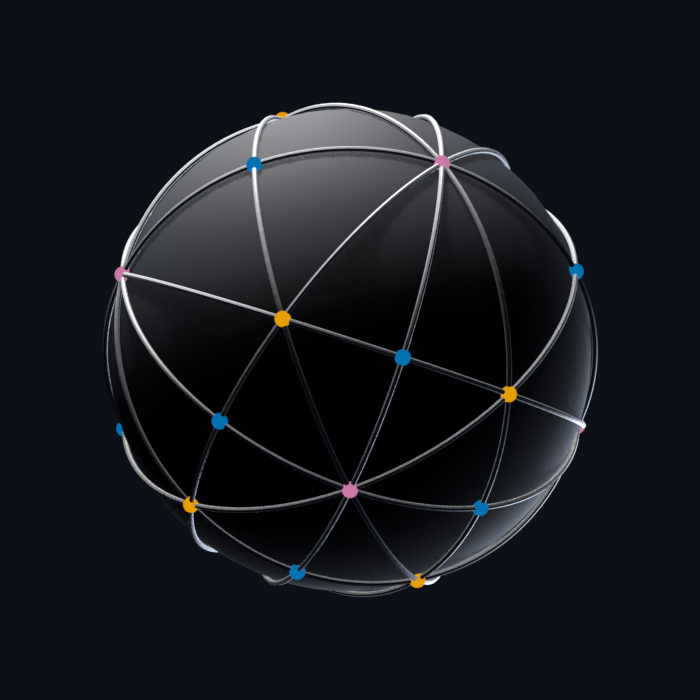
\includegraphics[width=0.48\textwidth]{figs/fig8_view_a.png}\hfill
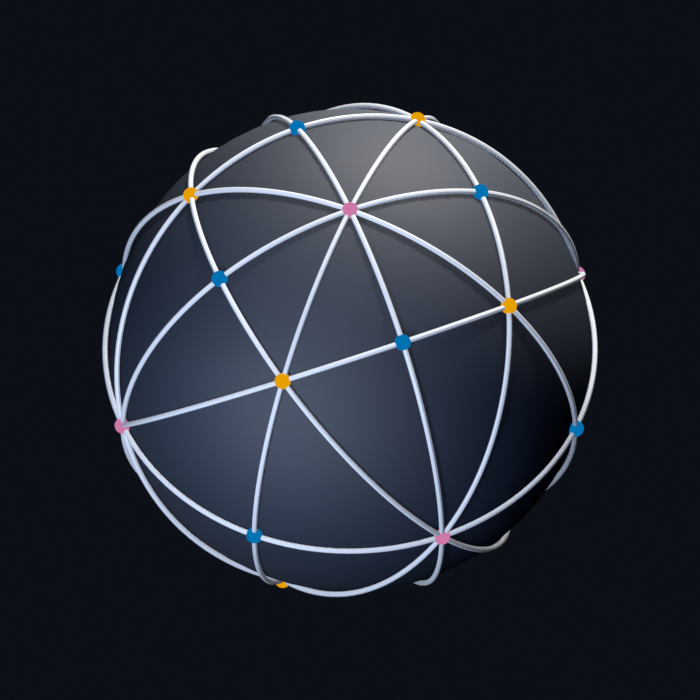
\includegraphics[width=0.48\textwidth]{figs/fig8_view_b.png}
\caption{An antipodal pair of orthographic views of the script's arrangement, chosen to maximise the smallest facing ($0.214$). Together they show all $26$ vertices; either alone shows $13$. The left view looks at the side the key light misses, so the globe is dark while the emissive markers keep their colours.}
\end{figure}

\section{A Shader Graph Is a Function}

A shader node graph is a small program with the same structure as the construction functions of Chapter 6: nodes are functions, links are composition, and the output node fixes what is returned to the renderer. The arrangement scene of Chapter 7 used three materials, one per multiplicity class, each a two-node graph with a constant colour. The same result can be obtained from one material whose colour is computed from data stored on the object. The Attribute node, with type Object and the name of a custom property, reads that property for the object being shaded and returns it as a number. A Map Range node rescales it, a Color Ramp with constant interpolation turns three levels into three colours, and the Emission shader outputs the result.

\Needspace{22\baselineskip}
\lstinputlisting[language=Python,basicstyle=\ttfamily\footnotesize,breaklines=true,frame=single,columns=fullflexible,keepspaces=true,firstline=89,lastline=104]{view_budget.py}

The single material has five nodes and four links. It was applied to every marker of the script's arrangement in place of the three class materials, and the scene was rendered twice at $450$ px and $16$ samples. Both renders contained the same connected regions of each class colour, $(8,5,3)$ for multiplicities $2$, $3$, $4$, and no pixel of the two images differed by more than two levels out of $255$, among $202{,}500$ pixels. The graph therefore reproduces the three-material result exactly in this scene. What it changes is where the information lives. In the three-material scene the class is stored twice, as a custom property and as a choice of material, and the two can disagree if one is edited. In the one-material scene the colour is a function of the property, so editing the property changes the colour, and a different arrangement needs only different property values. The cost is that the mapping from numbers to colours is hidden in the graph, so the ramp stops belong in the same record as the parameters, as Chapter 5 asks for modifier orders.

Two cautions follow from the measurement. First, the check shows that the graph matches the earlier material under Standard view transform and emission strength one; under another view transform both would change together, as Chapter 7 showed. Second, replacing the materials left the old three in the file as unused datablocks, so the scene file had six materials when only one was in use. This is the accumulation of Chapter 6 again, and the purge there applies.

\section{What a Render Costs}

A rendered image is the average of many samples per pixel, and the number of samples is a setting. Eevee's default for final renders is $64$. The effect of the setting on the result was measured on the script's arrangement at $300\times300$ pixels, taking a $256$-sample render as reference and reporting the root-mean-square difference over all pixels and channels, in levels out of $255$.

\begin{center}
\begin{tabular}{rrrr}
\toprule
Samples & RMS difference & Largest difference & Time (s)\\
\midrule
1 & 20.19 & 224 & 4\\
4 & 4.73 & 86 & 7\\
16 & 1.90 & 46 & 14\\
64 & 0.76 & 13 & 48\\
256 & (reference) & (reference) & 191\\
\bottomrule
\end{tabular}
\end{center}

Each fourfold increase in samples from $4$ to $64$ divided the RMS difference by about $2.5$, which is steeper than the factor of two that independent noise alone would give. The reference is itself a finite render, so the figures understate the true error, and the factor should not be read as a law. The largest single-pixel difference shows why an average hides what matters: at $16$ samples some pixel is still $46$ levels off, which is enough to move a marker's colour to another class on an eight-bit scale. The times for one and four samples come from the first measurement run and the others from a second run after a warm-up render, so the table is a rough guide; timings in this environment are specific to a software-rendered, windowless build, and they show a pattern more than a rate. Time grew about linearly with samples. It grew weakly with pixels: at $16$ samples, $300$, $600$, and $900$ pixels square took $14$, $18$, and $25$ seconds, so most of the cost of a small render was fixed per frame. A reader's machine will give different numbers, and the budget that matters is the one measured on the machine that will produce the final images.

Eevee proved deterministic in this configuration, on the evidence of two renders of the same scene with the same settings that were bit-identical, so a difference between two images could be attributed to a difference in the scene or in the settings and not to chance. Two renders are weak evidence, and Chapter 24 later found scenes in this same environment, with several hundred objects reading a material attribute at four samples, in which repeated renders of an unchanged scene were not identical. The property should therefore be checked, by repeated renders and a comparison of pixels, for each scene whose images are to be compared, and it is not guaranteed across hardware or Blender versions.

\section{Recording a Render}

The render budget is only comparable if the settings that produced an image are written down. The script below collects the settings that the measurements of this chapter and the last showed to matter: the Blender version, engine, resolution and resolution percentage, samples, view transform, look and exposure, the camera's type, focal length, sensor, orthographic scale, location and rotation, and the type and power of each light. It returns a dictionary that can be saved beside the image, and a short digest of the dictionary gives a quick equality test.

\Needspace{22\baselineskip}
\lstinputlisting[language=Python,basicstyle=\ttfamily\footnotesize,breaklines=true,frame=single,columns=fullflexible,keepspaces=true,firstline=8,lastline=26]{render_record.py}

On the script's arrangement the digest was \texttt{a55f051f3e2e}; setting the sample count to $16$ changed it to \texttt{17d9b2e75d7a}, and a second reading of an unchanged scene reproduced it. The record does not capture everything. It omits material parameters, mesh content, world colour, and the Python script itself, and a complete record would add the hash of the scene file and the commit of the construction script. It is the minimum that lets a reader say whether two renders were made under the same viewing conditions.

\section{What Was and Was Not Measured}

The measurements of this chapter establish that the pinhole formula and the field-of-view relation hold for the installed build, that half of the vertices of a centrally symmetric arrangement are hidden in every orthographic view, that three views reach every vertex of both arrangements at facing $0.2$, that one data-driven material reproduces three assigned materials in this scene, and that the sample count trades error against time in the measured way. They do not establish anything about Cycles, which was not available, about hardware-accelerated rendering, about lenses with distortion or depth of field, or about the interactive viewport. The camera comparison used point-like sources, so it says nothing about how well a thin line or a bevelled edge is localised. The sample study used a single scene and a single resolution.

\begin{exercise}[8.1: Fix the lights to the camera]
Parent the two lights of the arrangement scene to the camera and rerender the antipodal pair of Figure 8.1. Measure the mean brightness of the globe in the two views before and after, and state which change in the figure you would attribute to the lights and which to the geometry.
\end{exercise}

\begin{exercise}[8.2: A third view]
For the teaching arrangement, find a direction $\mathbf d_3$ that, added to the best antipodal pair, makes every vertex have facing above $0.2$ in at least one of the three views. Verify with a ray-cast in Blender that the centre bound then certifies as many of the $54$ markers as it can, and report the number.
\end{exercise}

\begin{exercise}[8.3: Edit the property, not the material]
Change the \texttt{multiplicity} property of one marker in the one-material scene and rerender. Confirm that its colour changed and that no material was edited. Then add a fourth class to the ramp, and write the sentence that a figure caption must contain so that a reader can recover the mapping.
\end{exercise}

\begin{exercise}[8.4: A budget for a figure]
Choose the smallest sample count at which the largest single-pixel difference from a $256$-sample reference is below $13$ levels for your own scene, and record the settings with the script of Section 8.5. State the machine on which the time was measured.
\end{exercise}
